\documentclass[a4]{article} 
\usepackage[czech]{babel} 
\usepackage[utf8]{inputenc} 
\usepackage{caption}
\usepackage{subcaption}
\usepackage{a4wide} 
\usepackage{amsmath,amsfonts,amssymb,amsthm}
\usepackage{graphicx}
\graphicspath{ {images/} }
\usepackage{float}
\usepackage{wrapfig}
\floatstyle{boxed} 
\restylefloat{figure}
\usepackage{geometry}
 \geometry{
 a4paper,
 left=40mm,
 top=25mm,
 bottom=25mm,
 right=25mm
 }



%TODO pridat geometry a udelat spravne okraje 
\begin{document} 
 
%titulni strana 
\begin{titlepage} 
\begin{center} 
{\huge\textsc{Gymnázium Jana Keplera}\\}
{\large{Praha 6, Parléřova 2}}\\
{\large{obor vzdělání Gymnázium 79-41-K/81}\\[5cm]} 
{\Large{Maturitní práce z informatiky}\\[0.2cm]}
{\Huge{Vývoj chůze pomocí\\neuroevolučních algoritmů}}\\\vfill
{\Large{Jan Bouček}\\} 
{\large{vedoucí práce: Tomáš Obdržálek}\\} 
{\large{Praha 2017}} 
\end{center} 
\end{titlepage} 
 
%prohlaseni 
\newpage 
Prohlašuji, že jsem jediným autorem této maturitní práce a všechny citace, použitá literatura a další zdroje jsou v práci uvedené. Tímto dle zákona 121/2000 Sb. (tzv. Autorský zákon) ve znění pozdějších předpisů uděluji bezúplatně škole Gymnázium Jana Keplera, Praha 6, Parléřova 2 oprávnění k výkonu práva na rozmnožování díla (§~13) a práva na sdělování díla veřejnosti (§~18) na dobu časově neomezenou a bez omezení územního rozsahu.\\[0.7cm] 
\vspace{10cm} 
{\large{V Praze dne 24. 3. 2017} \hfill Jan Bouček} 
%anotace 
\newpage 
\tableofcontents
\newpage
%TODO zrušit mezeru na začátku 
{\Large\textbf{Anotace}\par}
Jeden z problémů moderní robotiky je chůze, čehož se tato práce narozdíl od konvenčních metod snaží dosáhnout pomocí strojového učení, konkrétně neuroevolučního algoritmu s nepřímým kódováním. Ten za pomoci techniky HyperNEAT generuje simulaci primitivního mozku, který chůzi robota ovládá.\par 

{\Large\textbf{Annotation}\par}
One of the problems in modern robotics is robotic walking, which in this paper, unlike conventional methods, is achieved by machine learning, specifically using a neuroevolutionary algorithm with indirect encoding. The algorithm uses the HyperNEAT technique to generate a simulation of a primitive brain, which controls the gait of the robot.\par  

%samotna prace 
\title{Vývoj chůze pomocí neuroevolučních algoritmů} 
\author{Jan Bouček} 
\date{} 
\maketitle 
 
\section{Úvod} 
Jeden z cílů dnesšní robotiky je konstruovat roboty, kteří jsou všestranně využitelní díky své mobilitě. Toho lze dosáhnout různými způsoby, pro svou jednoduchost se často používá jízda, která ale neumožňuje spolehlivé zdolávání členitého terénu, nebo pohyb přímo ve strukturách stavěných člověkem, zejména pak zdolávání schodů.\par
Tato práce se inspiruje čtyřnohými kráčivými roboty firmy Boston Dynamics\cite{bostondynamics}, kteří dosahují stabilní chůze exaktními metodami.\cite{bdpaper} Podobné chůze by mělo být možné dosáhnout i pomocí organičtějších metod. Neuroevoluční algoritmy dokáží nabídnout přirozené řešení i na velmi komplexní problémy, či dokonce znovuobjevit řešení, které v přírodě už existuje, proto je možné generovat čtyřnohý pohyb i tímto způsobem.\cite{clunegait}\par
Cílem projektu pak je dosáhnout podobnou metodou stabilní, vzpřímené a repetitivní kupředné chůze na simulaci čtyřnohého robota.
 
\section{Teorie}
Chůzi lze definovat jakožto sérii stavů kráčivého tělesa, kde každý stav lze zjednodušit jako soubor informací popisující jednotlivé pohyblivé prvky robota. V rámci tohoto projektu budeme pracovat s dvojrozměrnou simulací čtyřnohého robota, jehož každá noha je ovládána dvěmi klouby. Stav robota tak lze vystihnout jako osmirozměrný vektor $\vec{s}$. Hledáme pak ovladač robota, který pro každý stav malezne osmirozměrný vektor $\vec{\omega}$, který každému kloubu určuje úhlovou rychlost.
\subsection{Evoluční algoritmy}
Evoluční algoritmy jsou metodou, která dokáže mnohnásobnou selekcí, mutací a kombinací různých řešení postupně vyvíjet optimálnější. K tomu potřebuje funkci, která dokáže každé řešení ohodnotit, tzv. \emph{fitness funkci}. V našem případě hodnotíme maximální vzdálenost robota od počátku směrem do kladných hodnot $x$, a vzhledem k tomu, že cílem je chůze vzpřímená, tak u každého řešení, ve kterém některý článek robota klesne svou výškou těžiště pod experimentálně zjištěnou hodnotu $Y_{min}$, nastavíme výslednou \emph{fitness} ovladače na \emph{0}.\par
Podobně jako v přírodě, evoluční algoritmus si udržuje \emph{populaci} řešení. V každém kroku ohodnotí výše zmíněnou funkcí každého \emph{živočicha}, podle své úspěšnosti jsou pak rozmnoženi (pohlavně, či nepohlavně) a zmutováni. Tento proces je podrobněji popsán v následující sekci.
\subsection{Neuroevoluce}
Neuroevoluční algoritmy jsou specifickou kategorií, která se zabývá trénováním umělých neuronových sítí, anglicky \emph{Artificial Neural Network} (ANN), které jsou abstraktním příblížením dějů v mozku, měly by být tedy schopné sloužit i jako ovladač našeho robota. Jejich struktura je popsána níže.
\subsubsection{Neuronové sítě}
Základní stavební jednotkou neuronové sítě je \emph{neuron}, ten je výpočetní jednotkou, která přijímá data ve formě spojů (z biologického hlediska \emph{dendrity}) s dalšími neurony. Pro každý z nich má nastavenou \emph{váhu} (anglicky \emph{weight}), která slouží jednoduše jako koeficient, který ovlivňuje \uv{důležitost} konkrétního spoje.\par
Výstupem, který pak mohou použít další neurony, je výsledek \emph{aktivační funkce} lineární kombinace hodnot napojených neuronů a příslušných vah\cite{neuron}:
\begin{center}$y_k=\phi(\sum_{j=0}^m w_{kj}\cdot x_j)$,\end{center}
kde $w$ je váha hodnoty neuronu $x$ a $\phi$ aktivační funkce.\par
Neurony pak lze tímto způsobem zapojovat do komplexnich sítí, kde hodnotu některých určujeme manuálně -- považujeme je za \emph{vstupy} sítě a u některých odečítáme hodnoty, čímž fungují jako \emph{výstupy} sítě.
\subsubsection{NEAT}
\emph{Neuroevolution of augmenting topologies}\cite{neat} (NEAT) je metodou, která definuje jeden ze způsobů, kterými lze vyvíjet neuronové sítě pomocí evolučního algoritmu. Revoluční ideou tohoto systému je způsob, kterým zapisuje neuronové sítě, jakožto \emph{živočicha}.\par
Každou neuronovou síť popisuje jako ohodnocený graf pomocí dvou seznamů \emph{genů} -- seznam vrcholů a seznam hran. Každému vrcholu a hraně přisuzuje číselné identifikároy, pomocí kterých je dokáže přehledně propojovat a udržovat přehled o tom, kteří jedinci jsou \uv{geneticky} podobní.\par
Stanley a Miikkulainen díky tomu zavádí i proces \emph{speciace}, který ještě před rozmnožováním roztřídí jedince do různých \emph{druhů} podle příbuznosti tak, aby se spolu křížily jen sítě s menšími rozdíly. Každý druh je pak ohodnocen svojí průměrnou hodnotou fitness, pomocí které se určí počet potomků v další generaci danného druhu.\par
Při procesu rozmnožování se z každého druhu vybere \emph{silnější} část, ze které se vytvoří požadovaný počet potomků, z nichž každý může vzniknout křížením -- většinu genů zdědí po silnějším rodiči, ale část od slabšího, nebo bez křížení, kdy se pouze jedinec zkopíruje do další generace.\par
Pak na všech potomcích proběhne mutace, přičemž je náhodně rozhodnuto, které z druhů mutací na něm proběhnou, Stanley a Miikkulainen popisují hned několik:
\begin{itemize}
\item{přidání nové hrany do sítě}
\item{rozdělení hrany na dvě hrany s novým neuronem uprostřed}
\item{změna všech vah o malou hodnotu, nebo na náhodnou hodnotu}
\end{itemize}
V tomto projektu je použito ještě několik dalších mutačních operátorů:
\begin{itemize}
\item{aktivace/deaktivace jedné hrany}
\item{změna jedné váhy na náhodnou hodnotu}
\item{změna jedné váhy o až $\pm 5\%$}
\end{itemize}
Díky této mírné úpravě dokáže algoritmus ladit neuronovou síť na trochu detailnějším měřítku.\par
Po zmutování jsou všichni potomci prohlášeni za současnou generaci a algoritmus pokračuje znovu hodnocením jedinců.
\subsection{CPPN-NEAT}
Tím, že v NEAT algoritmu umožníme každému neuronu využívat jinou aktivační funkci, můžeme dosáhnout sítí, které jsou dobře uzpůsobené ke generování fyzické geometrie živočichů. Metoda CPPN-NEAT\cite{cppn-neat} využívá různých vlastností funkcí -- symetrie, repetice apod. tak, že průchodem celou sítí jsou výsledná data nakombinována pomocí komplexní složené funkce, která si uchováva všechny tyto vlastnosti.\par
Pokud například vytvoříme CPPN síť s dvoumi vstupy -- souřadnice $x$ a $y$ s jedním výstupem, získáme dvojrozměrné útvary (viz obr. 1), které mají velmi blízko k fyzickému rozložení v reálných živočiších, např. dokáže nakombinovat repetici s variací a generovat útvary podobné prstům u ruky nebo pomocí symetrie a variace útvar podobný lidskému oku (viz obr. 1b)\par
V samotném algoritmu stačí jen při tvoření nových neuronů určit náhodnou aktivační funkci a přidat mutační operátor, který změní funkci u náhodného neuronu.\par

%https://en.wikibooks.org/wiki/LaTeX/Floats,_Figures_and_Captions#Subfloats
\begin{figure}
    \centering
    \begin{subfigure}[b]{0.3\textwidth}
        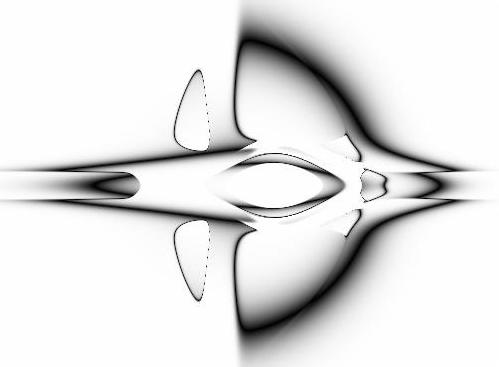
\includegraphics[width=\textwidth]{cppn1}
        \caption{symetrie}
        \label{fig:sym}
    \end{subfigure}
    ~ 
    \begin{subfigure}[b]{0.3\textwidth}
        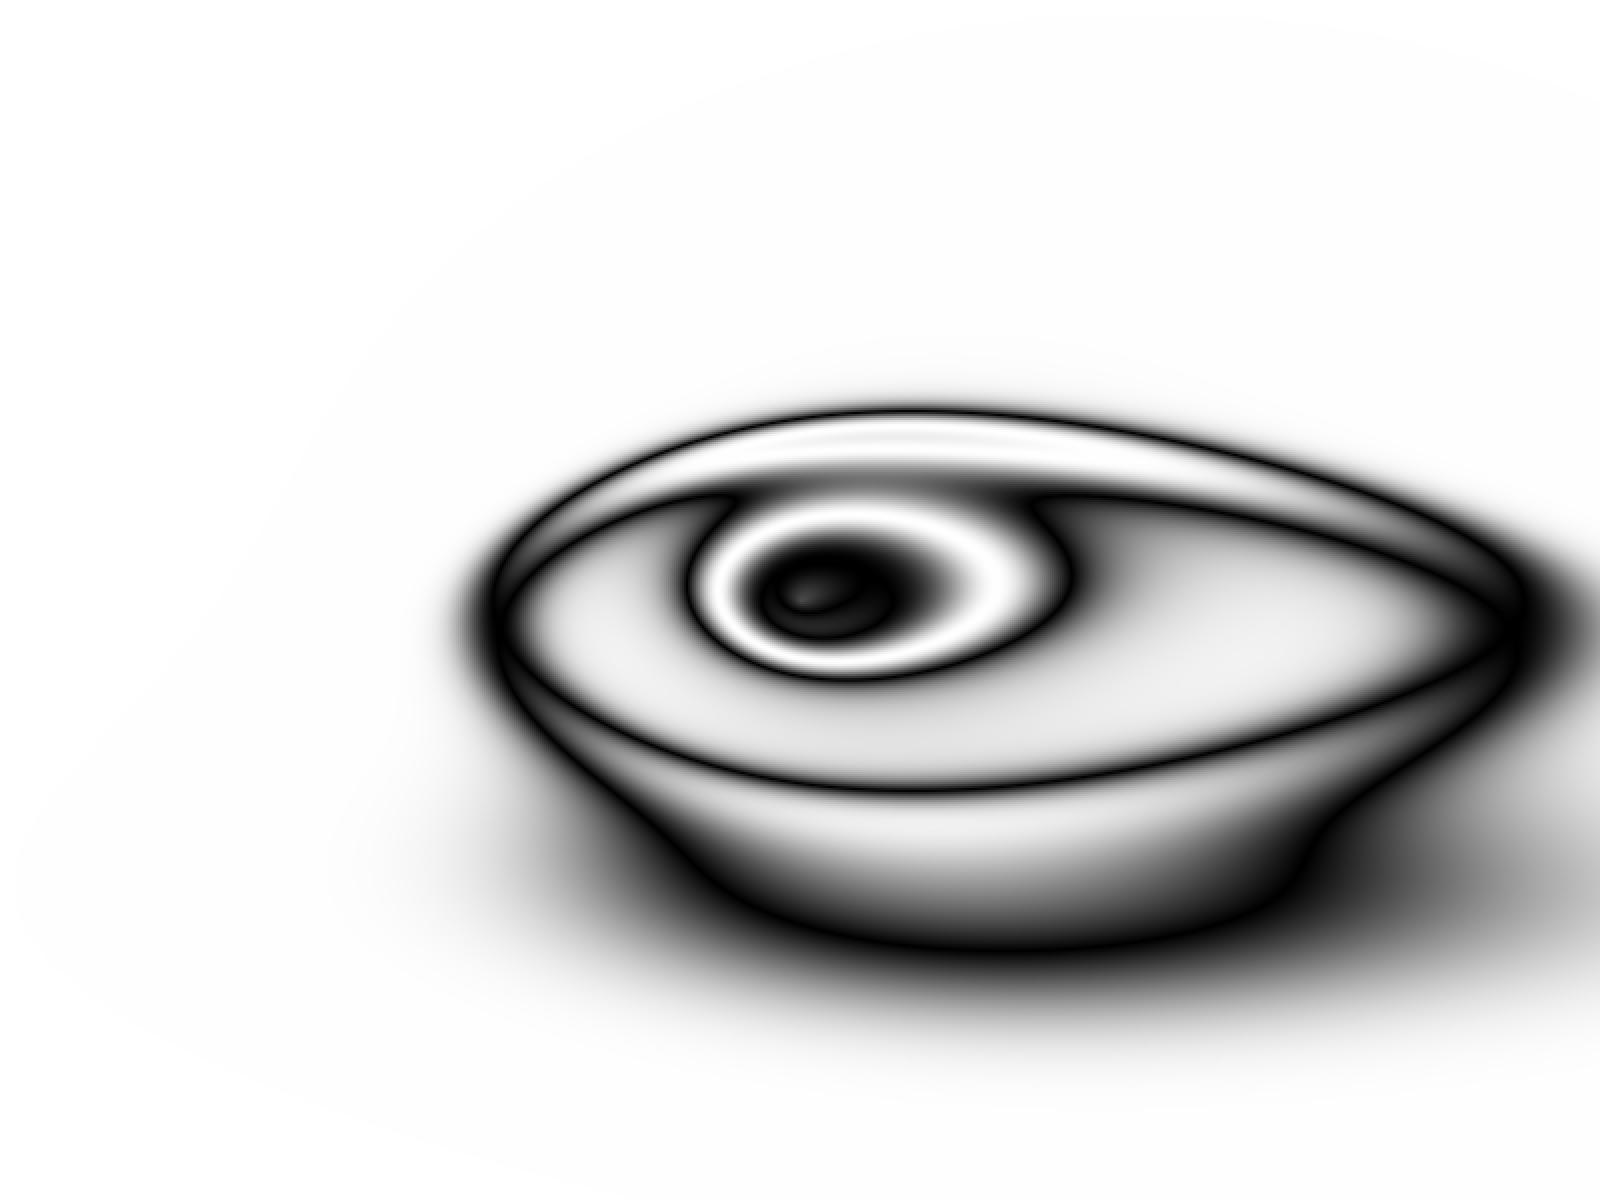
\includegraphics[width=\textwidth]{cppn2}
        \caption{nedokonalá symetrie}
        \label{fig:imperfectsym}
    \end{subfigure}
    ~ 
    \begin{subfigure}[b]{0.3\textwidth}
        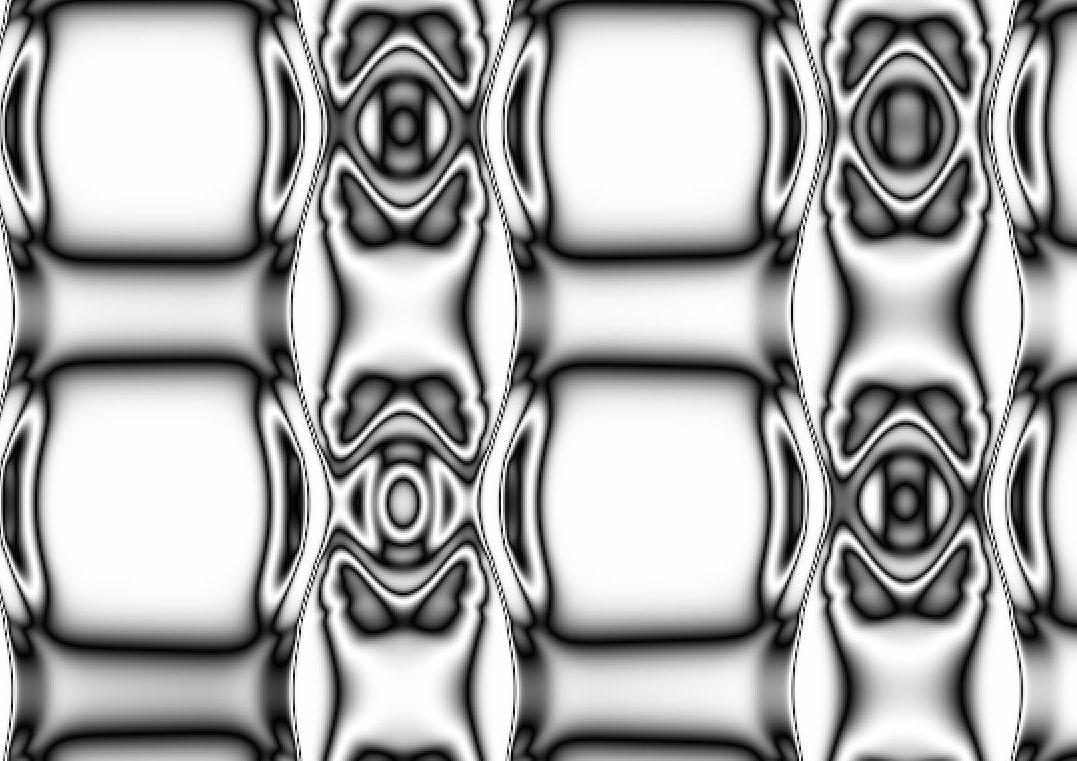
\includegraphics[width=\textwidth]{cppn3}
        \caption{repetice s variací}
        \label{fig:repvar}
    \end{subfigure}
    \caption{tvary vygenerované pomocí CPPN-NEAT, převzato\cite{hyperneat}}\label{fig:cppn}
\end{figure}
\subsection{HyperNEAT}
Technika HyperNEAT\cite{hyperneat} využívá CPPN sítě ke generování čtyřrozměrného prostoru, který ve výsledku slouží jako definice vah v další neuronové síti.\par
To znamená, že generujeme CPPN síť, která má čtyři vstupy -- $x_1$, $y_1$, $x_2$, $y_2$. Výstup nám pak určuje váhu spoje z neuronu na \emph{fyzických} souřadnicích $[x_1;y_1]$ do neuronu na souřadnicích $[x_2;y_2]$. Stačí nám pak vymyslet \emph{fyzickou} strukturu sítě, kterou využijeme této techniky.\par
V tomto projektu je použito rozložení zvané \emph{\uv{state-space sandwich}}\cite{hyperneat} o třech vrstvách podobně jako \cite{clunegait}, kde výsledná síť je rozvrstvená do trojrozměrného prostoru a z každého neuronu vede spoj do každého neuronu v další vrstvě. CPPN síť má pak dva výstupy, kde první určuje váhu mezi dannými souřadnicemi z první vrstvy do druhé a druhý výstup určuje váhy mezi druhou a třetí vrstvou.\par
\subsection{Rozložení sítě}
Narozdíl od klasických neuronových sítí jsou si sítě generované HyperNEATem \emph{vědomé} geometrických souvislostí\cite{hyperneat}, proto je naprosto zásadní rozmístění vstupů a výstupů ve výsledné síti.\par

\begin{wrapfigure}{r}{0.45\textwidth}
  \begin{center}
    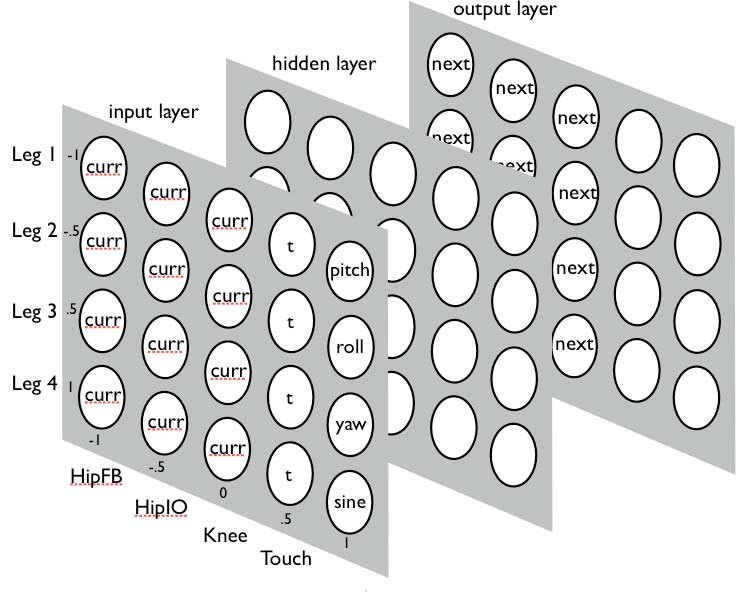
\includegraphics[width=0.4\textwidth]{clunenet}
  \end{center}
  \caption{rozložení sítě v \cite{clunegait}, převzato \cite{clunegait}}
\end{wrapfigure}
\cite{clunegait} umisťuje do každého řádku v \emph{substrátu} jednu nohu a do posledního sloupce přidává neuspořádaně zbylé informace (viz obr. 2).\par
Tento postup sice dává geometricky najevo související buňky -- podobné informace jsou ve stejných sloupcích, ale opomíjí rozložení nohou v prostoru, proto se v tomto projektu používá struktura, která za pomocí symetrie dává najevo souvislosti typu \emph{přední/zadní pár nohou} a \emph{levá/pravá noha}. Pro nejlepší výsledky je v rozložení nohou středová souměrnost a zbylé informace jsou v prostřední řadě mezi nohama. Každá noha je popsána pomocí dvou úhlů kloubů a dotykového \emph{senzoru} na spodním článku nohy, jehož hodnota je nastavena na $-1$ bez doteku a $1$ s dotekem, pro hladkost pohybu mají tyto hodnoty lineární přechod o délce 25 snímků.\par


\section{Výsledky} 
\section{Implementace?}%sem? 
\section{Závěr} 
\section{Uživatelská dokumentace} 
\section{Diskuze?}
\begin{thebibliography}{7}
\bibitem{bostondynamics}
Introducing Spot. In: \textit{Youtube} [online]. 9.2.2015 [cit. 2017-03-20]. Dostupné z: https://www.youtube.com/watch?v=M8YjvHYbZ9w. Kanál uživatele Boston Dynamics
\bibitem{bdpaper}RAIBERT, Marc, Kevin BLANKESPOOR, Gabriel NELSON a Rob PLAYTER. \textit{BigDog, the Rough-Terrain Quadruped Robot} [online]. [cit. 2017-03-20]. DOI: 10.3182/20080706-5-KR-1001.01833. ISBN 10.3182/20080706-5-KR-1001.01833. Dostupné z: http://linkinghub.elsevier.com/retrieve/pii/S1474667016407020
\bibitem{clunegait}
CLUNE, Jeff, Benjamin E. BECKMANN, Charles OFRIA a Robert T. PENNOCK. Evolving coordinated quadruped gaits with the HyperNEAT generative encoding. In: \textit{2009 IEEE Congress on Evolutionary Computation}. IEEE, 2009, s. 2764-2771. DOI: 10.1109/CEC.2009.4983289. ISBN 978-1-4244-2958-5. Dostupné také z: http://ieeexplore.ieee.org/document/4983289/
\bibitem{neuron}
Artificial neuron. In: \textit{Wikipedia: the free encyclopedia} [online]. San Francisco (CA): Wikimedia Foundation, 2001-2017 [cit. 2017-03-21]. Dostupné z: https://en.wikipedia.org/wiki/Artificial\_neuron
\bibitem{neat}
STANLEY, Kenneth O. a Risto MIIKKULAINEN. Evolving Neural Networks through Augmenting Topologies. \emph{Evolutionary Computation} [online]. 2002, \textbf{10}(2), 99-127 [cit. 2017-03-21]. DOI: 10.1162/106365602320169811. ISSN 1063-6560. Dostupné z: http://www.mitpressjournals.org/doi/10.1162/106365602320169811
\bibitem{cppn-neat}
STANLEY, Kenneth O. Compositional pattern producing networks: A novel abstraction of development. \emph{Genetic Programming and Evolvable Machines} [online]. 2007-6-6, \textbf{8}(2), 131-162 [cit. 2017-03-21]. DOI: 10.1007/s10710-007-9028-8. ISSN 1389-2576. Dostupné z: http://link.springer.com/10.1007/s10710-007-9028-8
\bibitem{hyperneat}
STANLEY, Kenneth O., David B. D'AMBROSIO a Jason GAUCI. A Hypercube-Based Encoding for Evolving Large-Scale Neural Networks. \textit{Artificial Life} [online]. 2009, \textbf{15}(2), 185-212 [cit. 2017-03-21]. DOI: 10.1162/artl.2009.15.2.15202. ISSN 1064-5462. Dostupné z: http://www.mitpressjournals.org/doi/10.1162/artl.2009.15.2.15202
\end{thebibliography}
\end{document}